%\documentclass{article}
%\usepackage{beamerarticle}
\documentclass[serif,ignorenonframetext]{beamer}

% Macros for MATH 110 course dates

\newcommand{\commonTheme}{metropolis}
\newcommand{\commonColorTheme}{metropolis}

\newcommand{\commonAuthor}{Edward Doolittle}
\newcommand{\commonInstitute}{Department of Indigenous Knowledge and
  Science \\ First Nations University of Canada}
\newcommand{\commonCourse}{MATH 110 Calculus I}
\newcommand{\commonTerm}{202510}
\newcommand{\commonDate}{January 6, 2025}

% Review Material

% Lab 0
\newcommand{\commonEventNegativeOne}{LabNegativeOne}
\newcommand{\commonDateLabNegativeOne}{Monday, January 6, 2025}
\newcommand{\commonTitleLabNegativeOne}{MATH 110 Lab 0}
\newcommand{\commonSubtitleLabNegativeOne}{No Lab; Course Opens}

% Section 001
\newcommand{\commonEventZeroZeroOne}{ZeroZeroOne}
\newcommand{\commonDateZeroZeroOne}{Tuesday, January 7, 2025}
\newcommand{\commonTitleZeroZeroOne}{MATH 110 Review 0.1}
\newcommand{\commonSubtitleZeroZeroOne}{Review of Algebra}
\newcommand{\commonPSTitleZeroZeroOne}{MATH 110 Review Problem Set 0.1}

% Section 00A
\newcommand{\commonEventZeroZeroA}{ZeroZeroA}
\newcommand{\commonDateZeroZeroA}{Tuesday, January 7, 2025}
\newcommand{\commonTitleZeroZeroA}{MATH 110 Review 0.A}
\newcommand{\commonSubtitleZeroZeroA}{Review of Inequalities and
  Absolute Values}
\newcommand{\commonPSTitleZeroZeroA}{MATH 110 Review Problem Set 0.A}

% Section 00B
\newcommand{\commonEventZeroZeroB}{ZeroZeroB}
\newcommand{\commonDateZeroZeroB}{Tuesday, January 7, 2025}
\newcommand{\commonTitleZeroZeroB}{MATH 110 Review 0.B}
\newcommand{\commonSubtitleZeroZeroB}{Review of Coordinate Geometry
  and Lines}
\newcommand{\commonPSTitleZeroZeroB}{MATH 110 Review Problem Set 0.B}

% Section 00C
\newcommand{\commonEventZeroZeroC}{ZeroZeroC}
\newcommand{\commonDateZeroZeroC}{Thursday, January 9, 2025}
\newcommand{\commonTitleZeroZeroC}{MATH 110 Review 0.C}
\newcommand{\commonSubtitleZeroZeroC}{Review of Graphs of Second
  Degree Equations}
\newcommand{\commonPSTitleZeroZeroC}{MATH 110 Review Problem Set 0.C}

% Section 00D
\newcommand{\commonEventZeroZeroD}{ZeroZeroD}
\newcommand{\commonDateZeroZeroD}{Thursday, January 9, 2025}
\newcommand{\commonTitleZeroZeroD}{MATH 110 Review 0.D}
\newcommand{\commonSubtitleZeroZeroD}{Review of Trigonometry}
\newcommand{\commonPSTitleZeroZeroD}{MATH 110 Review Problem Set 0.D}

% Section 011
\newcommand{\commonEventZeroOneOne}{ZeroOneOne}
\newcommand{\commonDateZeroOneOne}{Thursday, January 9, 2025}
\newcommand{\commonTitleZeroOneOne}{MATH 110 Review 1.1}
\newcommand{\commonSubtitleZeroOneOne}{Review of Functions}
\newcommand{\commonPSTitleZeroOneOne}{MATH 110 Review Problem Set 1.1}


% Main Course

% Lab 1
\newcommand{\commonEventZero}{LabZero}
\newcommand{\commonDateLabZero}{Monday, January 13, 2025}
\newcommand{\commonTitleLabZero}{MATH 110 Lab 1}
\newcommand{\commonSubtitleLabZero}{Quiz 0: STACK, Onboarding}

% Section 1.4
\newcommand{\commonEventOne}{ZeroOneFour}
\newcommand{\commonDateZeroOneFour}{Tuesday, January 14, 2025}
\newcommand{\commonTitleZeroOneFour}{MATH 110 Lecture 1.4}
\newcommand{\commonSubtitleZeroOneFour}{The Tangent and Velocity Problems}
\newcommand{\commonPSTitleZeroOneFour}{MATH 110 Problem Set 1.4}

% Section 1.5
\newcommand{\commonEventTwo}{ZeroOneFive}
\newcommand{\commonDateZeroOneFive}{Thursday, January 16, 2025}
\newcommand{\commonTitleZeroOneFive}{MATH 110 Lecture 1.5}
\newcommand{\commonSubtitleZeroOneFive}{The Limit of a Function}
\newcommand{\commonPSTitleZeroOneFive}{MATH 110 Problem Set 1.5}

% Lab 2
\newcommand{\commonEventThree}{LabOne}
\newcommand{\commonDateLabOne}{Monday, January 20, 2025}
\newcommand{\commonTitleLabOne}{MATH 110 Lab 2}
\newcommand{\commonSubtitleLabOne}{Quiz 1: Review}

% Section 1.6
\newcommand{\commonEventFour}{ZeroOneSix}
\newcommand{\commonDateZeroOneSix}{Tuesday, January 21, 2025}
\newcommand{\commonTitleZeroOneSix}{MATH 110 Lecture 1.6}
\newcommand{\commonSubtitleZeroOneSix}{Calculating Limits Using the Limit Laws}
\newcommand{\commonPSTitleZeroOneSix}{MATH 110 Problem Set 1.6}

% Section 1.7
\newcommand{\commonEventFive}{ZeroOneSeven}
\newcommand{\commonDateZeroOneSeven}{(Not covered)}
\newcommand{\commonTitleZeroOneSeven}{MATH 110 Lecture 1.7}
\newcommand{\commonSubtitleZeroOneSeven}{The Precise Definition of a Limit}
\newcommand{\commonPSTitleZeroOneSeven}{MATH 110 Problem Set 1.7}

% Section 1.8
\newcommand{\commonEventSix}{ZeroOneEight}
\newcommand{\commonDateZeroOneEight}{Thursday, January 23, 2025}
\newcommand{\commonTitleZeroOneEight}{MATH 110 Lecture 1.8}
\newcommand{\commonSubtitleZeroOneEight}{Continuity}
\newcommand{\commonPSTitleZeroOneEight}{MATH 110 Problem Set 1.8}

% Lab 3
\newcommand{\commonEventSeven}{LabTwo}
\newcommand{\commonDateLabTwo}{Monday, January 27, 2025}
\newcommand{\commonTitleLabTwo}{MATH 110 Lab 3}
\newcommand{\commonSubtitleLabTwo}{Quiz 2: Sections 1.4, 1.5}

% Section 2.1
\newcommand{\commonEventEight}{ZeroTwoOne}
\newcommand{\commonDateZeroTwoOne}{Tuesday, January 28, 2025}
\newcommand{\commonTitleZeroTwoOne}{MATH 110 Lecture 2.1}
\newcommand{\commonSubtitleZeroTwoOne}{Derivatives and Rates of Change}
\newcommand{\commonPSTitleZeroTwoOne}{MATH 110 Problem Set 2.1}

% Section 2.2
\newcommand{\commonEventNine}{ZeroTwoTwo}
\newcommand{\commonDateZeroTwoTwo}{Thursday, January 30, 2025}
\newcommand{\commonTitleZeroTwoTwo}{MATH 110 Lecture 2.2}
\newcommand{\commonSubtitleZeroTwoTwo}{The Derivative as a Function}
\newcommand{\commonPSTitleZeroTwoTwo}{MATH 110 Problem Set 2.2}

% Lab 4
\newcommand{\commonEventTen}{LabThree}
\newcommand{\commonDateMTOne}{Monday, February 3, 2025} 
\newcommand{\commonDateLabThree}{Monday, February 3, 2025}
\newcommand{\commonTitleLabThree}{MATH 110 Lab 4}
\newcommand{\commonSubtitleLabThree}{Midterm: Review, Chapter 1}

% Section 2.3
\newcommand{\commonEventEleven}{ZeroTwoThree}
\newcommand{\commonDateZeroTwoThree}{Tuesday, February 4, 2025}
\newcommand{\commonTitleZeroTwoThree}{MATH 110 Lecture 2.3}
\newcommand{\commonSubtitleZeroTwoThree}{Differentiation Formulas}
\newcommand{\commonPSTitleZeroTwoThree}{MATH 110 Problem Set 2.3}

% Section 2.4
\newcommand{\commonEventTwelve}{ZeroTwoFour}
\newcommand{\commonDateZeroTwoFour}{Thursday, February 6, 2025}
\newcommand{\commonTitleZeroTwoFour}{MATH 110 Lecture 2.4}
\newcommand{\commonSubtitleZeroTwoFour}{Derivatives of Trigonometric Functions}
\newcommand{\commonPSTitleZeroTwoFour}{MATH 110 Problem Set 2.4}

% Lab 5
\newcommand{\commonEventThirteen}{LabFour}
\newcommand{\commonDateLabFour}{Monday, February 10, 2025}
\newcommand{\commonTitleLabFour}{MATH 110 Lab 5}
\newcommand{\commonSubtitleLabFour}{Quiz 3: Sections 2.1, 2.2}

% Section 2.5
\newcommand{\commonEventFourteen}{ZeroTwoFive}
\newcommand{\commonDateZeroTwoFive}{Tuesday, February 11, 2025}
\newcommand{\commonTitleZeroTwoFive}{MATH 110 Lecture 2.5}
\newcommand{\commonSubtitleZeroTwoFive}{The Chain Rule}
\newcommand{\commonPSTitleZeroTwoFive}{MATH 110 Problem Set 2.5}

% Section 2.6
\newcommand{\commonEventFifteen}{ZeroTwoSix}
\newcommand{\commonDateZeroTwoSix}{Thursday, February 13, 2025}
\newcommand{\commonTitleZeroTwoSix}{MATH 110 Lecture 2.6}
\newcommand{\commonSubtitleZeroTwoSix}{Implicit Differentiation}
\newcommand{\commonPSTitleZeroTwoSix}{MATH 110 Problem Set 2.6}

% Lab 6
\newcommand{\commonEventSixteen}{LabFive}
\newcommand{\commonDateLabFive}{Monday, February 24, 2025}
\newcommand{\commonTitleLabFive}{MATH 110 Lab 6}
\newcommand{\commonSubtitleLabFive}{Quiz 4: Sections 2.3, 2.4}

% Section 2.7
\newcommand{\commonEventSeventeen}{ZeroTwoSeven}
\newcommand{\commonDateZeroTwoSeven}{Tuesday, February 25, 2025}
\newcommand{\commonTitleZeroTwoSeven}{MATH 110 Lecture 2.7}
\newcommand{\commonSubtitleZeroTwoSeven}{Rates of Change in the
  Natural and Social Sciences}
\newcommand{\commonPSTitleZeroTwoSeven}{MATH 110 Problem Set 2.7}

% Section 2.8
\newcommand{\commonEventEighteen}{ZeroTwoEight}
\newcommand{\commonDateZeroTwoEight}{Thursday, February 27, 2025}
\newcommand{\commonTitleZeroTwoEight}{MATH 110 Lecture 2.8}
\newcommand{\commonSubtitleZeroTwoEight}{Related Rates}
\newcommand{\commonPSTitleZeroTwoEight}{MATH 110 Problem Set 2.8}

% Lab 7
\newcommand{\commonEventNineteen}{LabSix}
\newcommand{\commonDateLabSix}{Monday, March 3, 2025}
\newcommand{\commonTitleLabSix}{MATH 110 Lab 7}
\newcommand{\commonSubtitleLabSix}{Quiz 5: Sections 2.5, 2.6}

% Section 3.1
\newcommand{\commonEventTwenty}{ZeroThreeOne}
\newcommand{\commonDateZeroThreeOne}{Tuesday, March 4, 2025}
\newcommand{\commonTitleZeroThreeOne}{MATH 110 Lecture 3.1}
\newcommand{\commonSubtitleZeroThreeOne}{Maximum and Minimum Values}
\newcommand{\commonPSTitleZeroThreeOne}{MATH 11 Problem Set 3.1}

% Section 3.2
\newcommand{\commonEventTwentyOne}{ZeroThreeTwo}
\newcommand{\commonDateZeroThreeTwo}{Thursday, March 6, 2025}
\newcommand{\commonTitleZeroThreeTwo}{MATH 110 Lecture 3.2}
\newcommand{\commonSubtitleZeroThreeTwo}{The Mean Value Theorem}
\newcommand{\commonPSTitleZeroThreeTwo}{MATH 110 Problem Set 3.2}

% Lab 8
\newcommand{\commonEventTwentyTwo}{LabSeven}
\newcommand{\commonDateMTTwo}{Monday, March 10, 2025}
\newcommand{\commonDateLabSeven}{Monday, March 10, 2025}
\newcommand{\commonTitleLabSeven}{MATH 110 Lab 8}
\newcommand{\commonSubtitleLabSeven}{Midterm: Chapter 2}

% Section 3.3
\newcommand{\commonEventTwentyThree}{ZeroThreeThree}
\newcommand{\commonDateZeroThreeThree}{Tuesday, March 11, 2025}
\newcommand{\commonTitleZeroThreeThree}{MATH 110 Lecture 3.3}
\newcommand{\commonSubtitleZeroThreeThree}{How Derivatives Affect the
  Shape of a Graph}
\newcommand{\commonPSTitleZeroThreeThree}{MATH 110 Problem Set 3.3}

% Section 3.4
\newcommand{\commonEventTwentyFour}{ZeroThreeFour}
\newcommand{\commonDateZeroThreeFour}{Thursday, March 13, 2025}
\newcommand{\commonTitleZeroThreeFour}{MATH 110 Lecture 3.4}
\newcommand{\commonSubtitleZeroThreeFour}{Limits at Infinity;
  Horizontal Asymptotes}
\newcommand{\commonPSTitleZeroThreeFour}{MATH 110 Problem Set 3.4}

% Lab 9
\newcommand{\commonEventTwentyFive}{LabEight}
\newcommand{\commonDateLabEight}{Monday, March 17, 2025}
\newcommand{\commonTitleLabEight}{MATH 110 Lab 9}
\newcommand{\commonSubtitleLabEight}{Quiz 6: Sections 3.1, 3.2}

% Section 3.5
\newcommand{\commonEventTwentySix}{ZeroThreeFive}
\newcommand{\commonDateZeroThreeFive}{Tuesday, March 18, 2025}
\newcommand{\commonTitleZeroThreeFive}{MATH 110 Lecture 3.5}
\newcommand{\commonSubtitleZeroThreeFive}{Summary of Curve Sketching}
\newcommand{\commonPSTitleZeroThreeFive}{MATH 110 Problem Set 3.5}

% Section 3.7
\newcommand{\commonEventTwentySeven}{ZeroThreeSeven}
\newcommand{\commonDateZeroThreeSeven}{Thursday, March 20, 2025}
\newcommand{\commonTitleZeroThreeSeven}{MATH 110 Lecture 3.7}
\newcommand{\commonSubtitleZeroThreeSeven}{Optimization Problems}
\newcommand{\commonPSTitleZeroThreeSeven}{MATH 110 Problem Set 3.7}

% Lab 10
\newcommand{\commonEventTwentyEight}{LabNine}
\newcommand{\commonDateLabNine}{Monday, March 24, 2025}
\newcommand{\commonTitleLabNine}{MATH 110 Lab 10}
\newcommand{\commonSubtitleLabNine}{Quiz 7: Sections 3.3, 3.4}

% Section 4.1
\newcommand{\commonEventTwentyNine}{ZeroFourOne}
\newcommand{\commonDateZeroFourOne}{Tuesday, March 25, 2025}
\newcommand{\commonTitleZeroFourOne}{MATH 110 Lecture 4.1}
\newcommand{\commonSubtitleZeroFourOne}{Areas and Distances}
\newcommand{\commonPSTitleZeroFourOne}{MATH 110 Problem Set 4.1}

% Section 4.2
\newcommand{\commonEventThirty}{ZeroFourTwo}
\newcommand{\commonDateZeroFourTwo}{Thursday, March 27, 2025}
\newcommand{\commonTitleZeroFourTwo}{MATH 110 Lecture 4.2}
\newcommand{\commonSubtitleZeroFourTwo}{The Definite Integral}
\newcommand{\commonPSTitleZeroFourTwo}{MATH 110 Problem Set 4.2}

% Lab 11
\newcommand{\commonEventThirtyOne}{LabTen}
\newcommand{\commonDateLabTen}{Monday, March 31, 2025}
\newcommand{\commonTitleLabTen}{MATH 110 Lab 11}
\newcommand{\commonSubtitleLabTen}{Quiz 8: Sections 3.5, 3.7}

% Section 4.3
\newcommand{\commonEventThirtyTwo}{ZeroFourThree}
\newcommand{\commonDateZeroFourThree}{Tuesday, April 1, 2025}
\newcommand{\commonTitleZeroFourThree}{MATH 110 Lecture 4.3}
\newcommand{\commonSubtitleZeroFourThree}{The Fundamental Theorem of Calculus}
\newcommand{\commonPSTitleZeroFourThree}{MATH 110 Problem Set 4.3}

% Section 4.4
\newcommand{\commonEventThirtyThree}{ZeroFourFour}
\newcommand{\commonDateZeroFourFour}{Thursday, April 3, 2025}
\newcommand{\commonTitleZeroFourFour}{MATH 110 Lecture 4.4}
\newcommand{\commonSubtitleZeroFourFour}{Indefinite Integrals and the
  Net Change Theorem}
\newcommand{\commonPSTitleZeroFourFour}{MATH 110 Problem Set 4.4}

% Lab 12
\newcommand{\commonEventThirtyFour}{LabEleven}
\newcommand{\commonDateLabEleven}{Monday, April 7, 2025}
\newcommand{\commonTitleLabEleven}{MATH 110 Lab 12}
\newcommand{\commonSubtitleLabEleven}{Quiz 9: Sections 4.1, 4.2}

% Section 4.5
\newcommand{\commonEventThirtyFive}{ZeroFourFive}
\newcommand{\commonDateZeroFourFive}{Tuesday, April 8, 2025}
\newcommand{\commonTitleZeroFourFive}{MATH 110 Lecture 4.5}
\newcommand{\commonSubtitleZeroFourFive}{The Substitution Rule}
\newcommand{\commonPSTitleZeroFourFive}{MATH 110 Problem Set 4.5}

% Section 5.1
\newcommand{\commonEventThirtySix}{ZeroFiveOne}
\newcommand{\commonDateZeroFiveOne}{Thursday, April 10, 2025}
\newcommand{\commonTitleZeroFiveOne}{MATH 110 Lecture 5.1}
\newcommand{\commonSubtitleZeroFiveOne}{Areas Between Curves}
\newcommand{\commonPSTitleZeroFiveOne}{MATH 110 Problem Set 5.1}

% Lab 13
\newcommand{\commonEventThirtySeven}{LabTwelve}
\newcommand{\commonDateLabTwelve}{Monday, April 14, 2025}
\newcommand{\commonTitleLabTwelve}{MATH 110 Review Lab}
\newcommand{\commonSubtitleLabTwelve}{Bonus Quiz 10: Sections 4.3, 4.4}

% Final Class
\newcommand{\commonEventThirtyEight}{FinalClass}
\newcommand{\commonDateFinalClass}{Tuesday, April 15, 2025}
\newcommand{\commonTitleFinalClass}{MATH 110 Review Class}
\newcommand{\commonSubtitleFinalClass}{Answer Questions, Review for Exam}

% Final Exam
\newcommand{\commonEventThirtyNine}{Final}
\newcommand{\commonDateFinal}{Thursday, April 22, 2025}
\newcommand{\commonTitleFinal}{MATH 110 Final Exam}
\newcommand{\commonSubtitleFinal}{Comprehensive Exam: All Sections}

% Orphaned -- no longer part of the course

% Section 2.9
\newcommand{\commonDateZeroTwoNine}{Not part of the course}
\newcommand{\commonTitleZeroTwoNine}{MATH 110 Lecture 2.9}
\newcommand{\commonSubtitleZeroTwoNine}{Linear Approximations and Differentials}
\newcommand{\commonPSTitleZeroTwoNine}{MATH 110 Problem Set 2.9}


% % Introduction
% \newcommand{\commonEventOneDate}{Wednesday, September 8, 2010}
% \newcommand{\commonEventOneDesc}{Introduction to the Course}
% \newcommand{\commonDateZeroZeroZero}{September 8, 2010}
% \newcommand{\commonTitleZeroZeroZero}{MATH 104 Introduction}
% \newcommand{\commonSubtitleZeroZeroZero}{Outline of the Course}

% % Lecture 1
% \newcommand{\commonEventTwoDate}{Friday, September 10, 2010}
% \newcommand{\commonEventTwoDesc}{Lecture 1: Algebra}
% \newcommand{\commonDateZeroZeroOne}{September 10, 2010}
% \newcommand{\commonTitleZeroZeroOne}{MATH 104 Lecture 1}
% \newcommand{\commonSubtitleZeroZeroOne}{Review of Algebra}
% % associated evaluation ... factor this out?
% \newcommand{\commonPSTitleZeroZeroOne}{MATH 104 Problem Set 1}
% \newcommand{\commonEvalZeroZeroOne}{Quiz 1}
% \newcommand{\commonEvalDateZeroZeroOne}{Wednesday, September 15, 2010}

% % Lecture 2
% \newcommand{\commonEventThreeDate}{Monday, September 13, 2010}
% \newcommand{\commonEventThreeDesc}{Lecture 2: Appendix A}
% \newcommand{\commonDateZeroZeroA}{September 13, 2010}
% \newcommand{\commonTitleZeroZeroA}{MATH 104 Lecture 2}
% \newcommand{\commonSubtitleZeroZeroA}{Appendix A: Numbers, Inequalities, 
%   and Absolute Values}
% % associated evaluation ... factor this out?
% \newcommand{\commonPSTitleZeroZeroA}{MATH 104 Problem Set 2}
% \newcommand{\commonEvalZeroZeroA}{Quiz 2}
% \newcommand{\commonEvalDateZeroZeroA}{Wednesday, September 22, 2010}

% % Review 1
% \newcommand{\commonEventFourDate}{Wednesday, September 15, 2010}
% \newcommand{\commonEventFourDesc}{Review 1: Review Algebra; Quiz 1; Review Appendix A}
% \newcommand{\commonDateRZeroOne}{September 15, 2010}
% \newcommand{\commonTitleRZeroOne}{MATH 104 Review 1}
% \newcommand{\commonSubtitleRZeroOne}{Review of Algebra, Appendix A}

% % Lecture 3
% \newcommand{\commonEventFiveDate}{Friday, September 17, 2010}
% \newcommand{\commonEventFiveDesc}{Lecture 3: Appendix B}
% \newcommand{\commonDateZeroZeroB}{September 17, 2010}
% \newcommand{\commonTitleZeroZeroB}{MATH 104 Lecture 3}
% \newcommand{\commonSubtitleZeroZeroB}{Appendix B: Coordinate Geometry and Lines}
% % associated evaluation ... factor this out?
% \newcommand{\commonPSTitleZeroZeroB}{MATH 104 Problem Set 3}
% \newcommand{\commonEvalZeroZeroB}{Quiz 2}
% \newcommand{\commonEvalDateZeroZeroB}{Wednesday, September 22, 2010}

% % Lecture 4
% \newcommand{\commonEventSixDate}{Monday, Sepbember 20, 2010}
% \newcommand{\commonEventSixDesc}{Lecture 4: Appendix C}
% \newcommand{\commonDateZeroZeroC}{September 20, 2010}
% \newcommand{\commonTitleZeroZeroC}{MATH 104 Lecture 4}
% \newcommand{\commonSubtitleZeroZeroC}{Appendix C: Graphs of Second-Degree Equations}
% % associated evaluation ... factor this out?
% \newcommand{\commonPSTitleZeroZeroC}{MATH 104 Problem Set 4}
% \newcommand{\commonEvalZeroZeroC}{Midterm 0}
% \newcommand{\commonEvalDateZeroZeroC}{Wednesday, September 29, 2010}

% % Review 2
% \newcommand{\commonEventSevenDate}{Wednesday, September 22, 2010}
% \newcommand{\commonEventSevenDesc}{Review 2: Review Appendix B; Quiz 2; Review Appendix C}
% \newcommand{\commonDateRZeroTwo}{September 22, 2010}
% \newcommand{\commonTitleRZeroTwo}{MATH 104 Review 2}
% \newcommand{\commonSubtitleRZeroTwo}{Review of Appendices B and C}

% % Lecture 5
% \newcommand{\commonEventEightDate}{Friday, September 24, 2010}
% \newcommand{\commonEventEightDesc}{Lecture 5: Appendix D}
% \newcommand{\commonDateZeroZeroD}{September 24, 2010}
% \newcommand{\commonTitleZeroZeroD}{MATH 104 Lecture 5}
% \newcommand{\commonSubtitleZeroZeroD}{Appendix D: Trigonometry}
% % associated evaluation ... factor this out?
% \newcommand{\commonPSTitleZeroZeroD}{MATH 104 Problem Set 5}
% \newcommand{\commonEvalZeroZeroD}{Midterm 0}
% \newcommand{\commonEvalDateZeroZeroD}{Wednesday, September 29, 2010}

% % Lecture 6
% \newcommand{\commonEventNineDate}{Monday, September 27, 2010}
% \newcommand{\commonEventNineDesc}{Lecture 6: Section 1.1}
% \newcommand{\commonDateZeroOneOne}{September 27, 2010}
% \newcommand{\commonTitleZeroOneOne}{MATH 104 Lecture 6}
% \newcommand{\commonSubtitleZeroOneOne}{Section 1.1: Four Ways to Represent a Function}
% % associated evaluation ... factor this out?
% \newcommand{\commonPSTitleZeroOneOne}{MATH 104 Problem Set 6}
% \newcommand{\commonEvalZeroOneOne}{Quiz 3}
% \newcommand{\commonEvalDateZeroOneOne}{Wednesday, October 6, 2010}

% % Review 3
% \newcommand{\commonEventTenDate}{Wednesday, September 29, 2010}
% \newcommand{\commonEventTenDesc}{Review 3: Review Appendix D; 
%   Self-Assessment Midterm 0}
% \newcommand{\commonDateRZeroThree}{September 29, 2010}
% \newcommand{\commonTitleRZeroThree}{MATH 104 Review 3}
% \newcommand{\commonSubtitleRZeroThree}{Review of Appendix D}

% % Lecture 7
% \newcommand{\commonEventElevenDate}{Friday, October 1, 2010}
% \newcommand{\commonEventElevenDesc}{Lecture 7: Section 1.2}
% \newcommand{\commonDateZeroOneTwo}{October 1, 2010}
% \newcommand{\commonTitleZeroOneTwo}{MATH 104 Lecture 7}
% \newcommand{\commonSubtitleZeroOneTwo}{Section 1.2: Mathematical Models: A Catalog of Essential Functions}
% % associated evaluation ... factor this out?
% \newcommand{\commonPSTitleZeroOneTwo}{MATH 104 Problem Set 7}
% \newcommand{\commonEvalZeroOneTwo}{Quiz 3}
% \newcommand{\commonEvalDateZeroOneTwo}{Wednesday, October 6, 2010}

% % Lecture 8
% \newcommand{\commonEventTwelveDate}{Monday, October 4, 2010}
% \newcommand{\commonEventTwelveDesc}{Lecture 8: Section 1.3}
% \newcommand{\commonDateZeroOneThree}{October 4, 2010}
% \newcommand{\commonTitleZeroOneThree}{MATH 104 Lecture 8}
% \newcommand{\commonSubtitleZeroOneThree}{Section 1.3: New Functions from Old Functions}
% % associated evaluation ... factor this out?
% \newcommand{\commonPSTitleZeroOneThree}{MATH 104 Problem Set 8}
% \newcommand{\commonEvalZeroOneThree}{Quiz 4}
% \newcommand{\commonEvalDateZeroOneThree}{Wednesday, October 13, 2010}

% % Review 4
% \newcommand{\commonEventThirteenDate}{Wednesday, October 6, 2010}
% \newcommand{\commonEventThirteenDesc}{Review 4: Review 1.1, 1.2; Quiz 3}
% \newcommand{\commonDateROneOne}{October 6, 2010}
% \newcommand{\commonTitleROneOne}{MATH 104 Review 4}
% \newcommand{\commonSubtitleROneOne}{Reveiw of 1.1, 1.2}

% % Lecture 9
% \newcommand{\commonEventFourteenDate}{Friday, October 8, 2010}
% \newcommand{\commonEventFourteenDesc}{Lecture 9: Section 1.4}
% \newcommand{\commonDateZeroOneFour}{October 8, 2010}
% \newcommand{\commonTitleZeroOneFour}{MATH 104 Lecture 9}
% \newcommand{\commonSubtitleZeroOneFour}{Section 1.4: Graphing Calculators and Computers}
% % associated evaluation ... factor this out?
% \newcommand{\commonPSTitleZeroOneFour}{MATH 104 Problem Set 9}
% \newcommand{\commonEvalZeroOneFour}{Quiz 4}
% \newcommand{\commonEvalDateZeroOneFour}{Wednesday, October 13, 2010}

% % Thanksgiving holiday
% \newcommand{\commonEventFifteenDate}{Monday, October 11, 2010}
% \newcommand{\commonEventFifteenDesc}{No class: Thanksgiving holiday}

% % Review 5
% \newcommand{\commonEventSixteenDate}{Wednesday, October 13, 2010}
% \newcommand{\commonEventSixteenDesc}{Review 5: Review 1.3, 1.4; Quiz 4}
% \newcommand{\commonDateROneTwo}{October 13, 2010}
% \newcommand{\commonTitleROneTwo}{MATH 104 Review 5}
% \newcommand{\commonSubtitleOneRTwo}{Review of 1.3, 1.4}

% % Lecture 10
% \newcommand{\commonEventSeventeenDate}{Friday, October 15, 2010}
% \newcommand{\commonEventSeventeenDesc}{Lecture 10: Section 1.5}
% \newcommand{\commonDateZeroOneFive}{October 15, 2010}
% \newcommand{\commonTitleZeroOneFive}{MATH 104 Lecture 10}
% \newcommand{\commonSubtitleZeroOneFive}{Section 1.5: Exponential Functions}
% % associated evaluation ... factor this out?
% \newcommand{\commonPSTitleZeroOneFive}{MATH 104 Problem Set 10}
% \newcommand{\commonEvalZeroOneFive}{Quiz 5}
% \newcommand{\commonEvalDateZeroOneFive}{Wednesday, October 20, 2010}

% % Lecture 11
% \newcommand{\commonEventEighteenDate}{Monday, October 18, 2010}
% \newcommand{\commonEventEighteenDesc}{Lecture 11: Section 1.6}
% \newcommand{\commonDateZeroOneSix}{October 18, 2010}
% \newcommand{\commonTitleZeroOneSix}{MATH 104 Lecture 11}
% \newcommand{\commonSubtitleZeroOneSix}{Section 1.6: Inverse Functions and Logarithms}
% % associated evaluation ... factor this out?
% \newcommand{\commonPSTitleZeroOneSix}{MATH 104 Problem Set 11}
% \newcommand{\commonEvalZeroOneSix}{Midterm 1}
% \newcommand{\commonEvalDateZeroOneSix}{Wednesday, October 27, 2010}

% % Review 6
% \newcommand{\commonEventNineteenDate}{Wednesday, October 20, 2010}
% \newcommand{\commonEventNineteenDesc}{Review 6: Review 1.5; Quiz 5; Review 1.6}
% \newcommand{\commonDateROneThree}{October 20, 2010}
% \newcommand{\commonDateZeroOneR}{October 20, 2010}
% \newcommand{\commonTitleROneThree}{MATH 104 Review 6}
% \newcommand{\commonSubtitleROneThree}{Review of 1.5, 1.6}
% % associated evaluation ... factor this out?
% \newcommand{\commonPSTitleZeroOneR}{MATH 104 Problem Set R1}
% \newcommand{\commonEvalZeroOneR}{Midterm 1}
% \newcommand{\commonEvalDateZeroOneR}{Wednesday, October 27, 2010}

% % Lecture 12
% \newcommand{\commonEventTwentyDate}{Friday, October 22, 2010}
% \newcommand{\commonEventTwentyDesc}{Lecture 12: Section 2.1}
% \newcommand{\commonDateZeroTwoOne}{October 22, 2010}
% \newcommand{\commonTitleZeroTwoOne}{MATH 104 Lecture 12}
% \newcommand{\commonSubtitleZeroTwoOne}{Section 2.1: The Tangent and Velocity Problems}
% % associated evaluation ... factor this out?
% \newcommand{\commonPSTitleZeroTwoOne}{MATH 104 Problem Set 12}
% \newcommand{\commonEvalZeroTwoOne}{Quiz 6}
% \newcommand{\commonEvalDateZeroTwoOne}{Wednesday, November 3, 2010}

% % Lecture 13
% \newcommand{\commonEventTwentyOneDate}{Monday, October 25, 2010}
% \newcommand{\commonEventTwentyOneDesc}{Lecture 13: Section 2.2(a)}
% \newcommand{\commonDateZeroTwoTwoa}{October 25, 2010}
% \newcommand{\commonTitleZeroTwoTwoa}{MATH 104 Lecture 13}
% \newcommand{\commonSubtitleZeroTwoTwoa}{Section 2.2(a): The Limit of a Function I}
% % associated evaluation ... factor this out?
% \newcommand{\commonPSTitleZeroTwoTwoa}{MATH 104 Problem Set 13}
% \newcommand{\commonEvalZeroTwoTwoa}{Quiz 6}
% \newcommand{\commonEvalDateZeroTwoTwoa}{Wednesday, November 3, 2010}

% % Midterm Test 1
% % October 27, 2010
% \newcommand{\commonEventTwentyTwoDate}{Wednesday, October 27, 2010}
% \newcommand{\commonEventTwentyTwoDesc}{Midterm Test 1: Chapter 1}

% % Lecture 14
% \newcommand{\commonEventTwentyThreeDate}{Friday, October 29, 2010}
% \newcommand{\commonEventTwentyThreeDesc}{Lecture 14: Section 2.2(b)}
% \newcommand{\commonDateZeroTwoTwob}{October 29, 2010}
% \newcommand{\commonTitleZeroTwoTwob}{MATH 104 Lecture 14}
% \newcommand{\commonSubtitleZeroTwoTwob}{Section 2.2(b): The Limit of a Function II}
% % associated evaluation ... factor this out?
% \newcommand{\commonPSTitleZeroTwoTwob}{MATH 104 Problem Set 14}
% \newcommand{\commonEvalZeroTwoTwob}{Quiz 6}
% \newcommand{\commonEvalDateZeroTwoTwob}{Wednesday, November 3, 2010}

% % Lecture 15
% \newcommand{\commonEventTwentyFourDate}{Monday, November 1, 2010}
% \newcommand{\commonEventTwentyFourDesc}{Lecture 15: Section 2.3}
% \newcommand{\commonDateZeroTwoThree}{November 1, 2010}
% \newcommand{\commonTitleZeroTwoThree}{MATH 104 Lecture 15}
% \newcommand{\commonSubtitleZeroTwoThree}{Section 2.3: Calculating Limits Using the Limit Laws}
% % associated evaluation ... factor this out?
% \newcommand{\commonPSTitleZeroTwoThree}{MATH 104 Problem Set 15}
% \newcommand{\commonEvalZeroTwoThree}{Quiz 7}
% \newcommand{\commonEvalDateZeroTwoThree}{Wednesday, November 10, 2010}

% % Review 7
% \newcommand{\commonEventTwentyFiveDate}{Wednesday, November 3, 2010}
% \newcommand{\commonEventTwentyFiveDesc}{Review 7: Review 2.1, 2.2; Quiz 6; Review 2.3}
% \newcommand{\commonDateRTwoOne}{November 3, 2010}
% \newcommand{\commonTitleRTwoOne}{MATH 104 Review 7}
% \newcommand{\commonSubtitleRTwoOne}{Review of 2.1, 2.2, 2.3}

% % Lecture 16
% \newcommand{\commonEventTwentySixDate}{Friday, November 5, 2010}
% \newcommand{\commonEventTwentySixDesc}{Lecture 16: Section 2.5}
% \newcommand{\commonDateZeroTwoFive}{November 5, 2010}
% \newcommand{\commonTitleZeroTwoFive}{MATH 104 Lecture 16}
% \newcommand{\commonSubtitleZeroTwoFive}{Section 2.5: Continuity}
% % associated evaluation ... factor this out?
% \newcommand{\commonPSTitleZeroTwoFive}{MATH 104 Problem Set 16}
% \newcommand{\commonEvalZeroTwoFive}{Quiz 7}
% \newcommand{\commonEvalDateZeroTwoFive}{Wednesday, November 10, 2010}

% % Lecture 17
% \newcommand{\commonEventTwentySevenDate}{Monday, November 8, 2010}
% \newcommand{\commonEventTwentySevenDesc}{Lecture 17: Section 2.6}
% \newcommand{\commonDateZeroTwoSix}{November 8, 2010}
% \newcommand{\commonTitleZeroTwoSix}{MATH 104 Lecture 17}
% \newcommand{\commonSubtitleZeroTwoSix}{Section 2.6: Limits at Infinity: Horizontal Asymptotes}
% % associated evaluation ... factor this out?
% \newcommand{\commonPSTitleZeroTwoSix}{MATH 104 Problem Set 17}
% \newcommand{\commonEvalZeroTwoSix}{Quiz 8}
% \newcommand{\commonEvalDateZeroTwoSix}{Wednesday, November 17, 2010}

% % Review 8
% \newcommand{\commonEventTwentyEightDate}{Wednesday, November 10, 2010}
% \newcommand{\commonEventTwentyEightDesc}{Review 8: Review 2.5; Quiz 7; Review 2.6}
% \newcommand{\commonDateRTwoTwo}{November 10, 2010}
% \newcommand{\commonTitleRTwoTwo}{MATH 104 Review 8}
% \newcommand{\commonSubtitleRTwoTwo}{Review of 2.5, 2.6}

% % Lecture 18
% \newcommand{\commonEventTwentyNineDate}{Friday, November 12, 2010}
% \newcommand{\commonEventTwentyNineDesc}{Lecture 18: Section 2.7}
% \newcommand{\commonDateZeroTwoSeven}{November 12, 2010}
% \newcommand{\commonTitleZeroTwoSeven}{MATH 104 Lecture 18}
% \newcommand{\commonSubtitleZeroTwoSeven}{Section 2.7: Derivatives and Rates of Change}
% % associated evaluation ... factor this out?
% \newcommand{\commonPSTitleZeroTwoSeven}{MATH 104 Problem Set 18}
% \newcommand{\commonEvalZeroTwoSeven}{Quiz 8}
% \newcommand{\commonEvalDateZeroTwoSeven}{Wednesday, November 17, 2010}

% % Lecture 19
% \newcommand{\commonEventThirtyDate}{Monday, November 15, 2010}
% \newcommand{\commonEventThirtyDesc}{Lecture 19: Section 2.8}
% \newcommand{\commonDateZeroTwoEight}{November 15, 2010}
% \newcommand{\commonTitleZeroTwoEight}{MATH 104 Lecture 19}
% \newcommand{\commonSubtitleZeroTwoEight}{Section 2.8: The Derivative as a Function}
% % associated evaluation ... factor this out?
% \newcommand{\commonPSTitleZeroTwoEight}{MATH 104 Problem Set 19}
% \newcommand{\commonEvalZeroTwoEight}{Midterm 2}
% \newcommand{\commonEvalDateZeroTwoEight}{Wednesday, November 24, 2010}

% % Review 9
% % November 17, 2010
% \newcommand{\commonEventThirtyOneDate}{Wednesday, November 17, 2010}
% \newcommand{\commonEventThirtyOneDesc}{Review 9: Review 2.7; Quiz 8; Review 2.8}
% \newcommand{\commonDateRTwoThree}{November 17, 2010}
% \newcommand{\commonTitleRTwoThree}{MATH 104 Review 9}
% \newcommand{\commonSubtitleRTwoThree}{Review of 2.7, 2.8}

% % Lecture 20
% \newcommand{\commonEventThirtyTwoDate}{Friday, November 19, 2010}
% \newcommand{\commonEventThirtyTwoDesc}{Lecture 20: Section 3.1}
% \newcommand{\commonDateZeroThreeOne}{November 19, 2010}
% \newcommand{\commonTitleZeroThreeOne}{MATH 104 Lecture 20}
% \newcommand{\commonSubtitleZeroThreeOne}{Section 3.1: Derivatives of Polynomials and Exponential Functions}
% % associated evaluation ... factor this out?
% \newcommand{\commonPSTitleZeroThreeOne}{MATH 104 Problem Set 20}
% \newcommand{\commonEvalZeroThreeOne}{Quiz 9}
% \newcommand{\commonEvalDateZeroThreeOne}{Wednesday, December 1, 2010}

% % Lecture 21
% \newcommand{\commonEventThirtyThreeDate}{Monday, November 22, 2010}
% \newcommand{\commonEventThirtyThreeDesc}{Lecture 21: Section 3.2}
% \newcommand{\commonDateZeroThreeTwo}{November 22, 2010}
% \newcommand{\commonTitleZeroThreeTwo}{MATH 104 Lecture 21}
% \newcommand{\commonSubtitleZeroThreeTwo}{Section 3.2: The Product and Quotient Rules}
% % associated evaluation ... factor this out?
% \newcommand{\commonPSTitleZeroThreeTwo}{MATH 104 Problem Set 21}
% \newcommand{\commonEvalZeroThreeTwo}{Quiz 9}
% \newcommand{\commonEvalDateZeroThreeTwo}{Wednesday, December 1, 2010}

% % Midterm Test 2
% \newcommand{\commonEventThirtyFourDate}{Wednesday, November 24, 2010}
% \newcommand{\commonEventThirtyFourDesc}{Midterm Test 2: Chapter 2}

% % Lecture 22
% \newcommand{\commonEventThirtyFiveDate}{Friday, November 26, 2010}
% \newcommand{\commonEventThirtyFiveDesc}{Lecture 22: Section 3.3}
% \newcommand{\commonDateZeroThreeThree}{November 26, 2010}
% \newcommand{\commonTitleZeroThreeThree}{MATH 104 Lecture 22}
% \newcommand{\commonSubtitleZeroThreeThree}{Section 3.3: Derivatives of Trigonometric Functions}
% % associated evaluation ... factor this out?
% \newcommand{\commonPSTitleZeroThreeThree}{MATH 104 Problem Set 22}
% \newcommand{\commonEvalZeroThreeThree}{Quiz 9}
% \newcommand{\commonEvalDateZeroThreeThree}{Wednesday, December 1, 2010}

% % Lecture 23
% \newcommand{\commonEventThirtySixDate}{Monday, November 29, 2010}
% \newcommand{\commonEventThirtySixDesc}{Lecture 23: Section 3.4}
% \newcommand{\commonDateZeroThreeFour}{November 29, 2010}
% \newcommand{\commonTitleZeroThreeFour}{MATH 104 Lecture 23}
% \newcommand{\commonSubtitleZeroThreeFour}{Section 3.4: The Chain Rule}
% % associated evaluation ... factor this out?
% \newcommand{\commonPSTitleZeroThreeFour}{MATH 104 Problem Set 23}
% \newcommand{\commonEvalZeroThreeFour}{the final exam}
% \newcommand{\commonEvalDateZeroThreeFour}{Monday, December 13, 2010}

% % Review 10
% \newcommand{\commonEventThirtySevenDate}{Wednesday, December 1, 2010}
% \newcommand{\commonEventThirtySevenDesc}{Review 10: Review 3.1, 3.2, 3.3; Quiz 9}
% \newcommand{\commonDateRThreeTwo}{December 1, 2010}
% \newcommand{\commonTitleRThreeTwo}{MATH 104 Review 10}
% \newcommand{\commonSubtitleRThreeTwo}{Review of 3.1, 3.2, 3.3}

% % Lecture 24
% \newcommand{\commonEventThirtyEightDate}{Friday, December 3, 2010}
% \newcommand{\commonEventThirtyEightDesc}{Lecture 24: Section 3.5}
% \newcommand{\commonDateZeroThreeFive}{December 3, 2010}
% \newcommand{\commonTitleZeroThreeFive}{MATH 104 Lecture 24}
% \newcommand{\commonSubtitleZeroThreeFive}{Section 3.5: Implicit Differentiation}
% % associated evaluation ... factor this out?
% \newcommand{\commonPSTitleZeroThreeFive}{MATH 104 Problem Set 24}
% \newcommand{\commonEvalZeroThreeFive}{the final exam}
% \newcommand{\commonEvalDateZeroThreeFive}{Monday, December 13, 2010}

% % Lecture 25
% \newcommand{\commonEventThirtyNineDate}{Monday, December 6, 2010}
% \newcommand{\commonEventThirtyNineDesc}{Lecture 25: Section 3.6}
% \newcommand{\commonDateZeroThreeSix}{December 6, 2010}
% \newcommand{\commonTitleZeroThreeSix}{MATH 104 Lecture 25}
% \newcommand{\commonSubtitleZeroThreeSix}{Section 3.6: Derivatives of Logarithmic Functions}
% % associated evaluation ... factor this out?
% \newcommand{\commonPSTitleZeroThreeSix}{MATH 104 Problem Set 25}
% \newcommand{\commonEvalZeroThreeSix}{the final exam}
% \newcommand{\commonEvalDateZeroThreeSix}{Monday, December 13, 2010}

% % Review 11
% \newcommand{\commonEventFortyDate}{Wednesday, December 8, 2010}
% \newcommand{\commonEventFortyDesc}{(Bonus) Review 11: Review 3.4, 3.5, 3.6}
% \newcommand{\commonDateRThreeThree}{December 8, 2010}
% \newcommand{\commonTitleRThreeThree}{MATH 104 (Bonus) Review 11}
% \newcommand{\commonSubtitleRThreeThree}{Review of 3.4, 3.5, 3.6}

% % Final Exam
% % December 13, 2010
% \newcommand{\commonEventFinalDate}{Monday, December 13, 2010}
% \newcommand{\commonEventFinalDesc}{MATH 104 Final Exam}

%%% Local variables:
%%% mode: latex
%%% TeX-master: "MATH110-Syllabus.tex"
%%% End:

\usepackage{mathptmx}
\usepackage{multirow}
\usepackage{tikz}

\newcommand{\ds}{\displaystyle}

\mode<article>{}
\mode<presentation>{\usetheme{\commonTheme}\usecolortheme{\commonColorTheme}}

\title{\commonTitleZeroZeroB}
\subtitle{\commonSubtitleZeroZeroB}
\author{\commonAuthor}
\institute{\commonInstitute}
\date{\commonDateZeroZeroB}

\begin{document}

%\section*{Outline}

\begin{frame}
  \titlepage
\end{frame}

\begin{frame}
  \frametitle{Contents}
  \tableofcontents
\end{frame}


\section{Coordinate Geometry and Lines}

\subsection{The Cartesian Coordinate System}

% EJD: graphics bounce around
\begin{frame}
  \frametitle{Cartesian Coordinates}
  \begin{columns}
    \column{0.65\textwidth}
    \begin{itemize}[<+->]
    \item<1-> The big idea of Cartesian coordinates is using a pair of
      numbers to locate points on the plane.
    \item<2-> We start with two perpendicular lines called ``axes'',
      through an ``origin'' $O$.
    \item<3-> Given a point on the plane ...
    \item<4-> we measure the distance to the vertical axis ...
    \item<5-> and to the horizontal axis ...
    \item<6-> which become the $(x,y)$ coordinates of the point.
    \end{itemize}
    \column{0.35\textwidth}
    \only<1>{%
      \begin{tikzpicture}
        %\draw[very thin,gray,step=0.5] (-1.75,-1.75) grid
        %(1.75,1.75); 
        \draw[->,transparent] (-1.75,0) -- (1.75,0) ; % node[above]{$x$} ; 
        \draw[->,transparent] (0,-1.75) -- (0,1.75) ; % node[right]{$y$} ;
        \draw[color=black,fill=black,transparent] (0,0) circle (0.05)
          node[below left] {$O$} ; 
        \draw[color=red,fill=red,transparent] (0.75,1.25) circle (0.05) node[right] {$P$} ;
        \draw[<->,very thin,color=red,transparent] (0,1.25) -- (0.75,1.25);
        \draw[<->,very thin,color=red,transparent] (0.75,0) -- (0.75,1.25);
      \end{tikzpicture}%
    }
    \only<2>{%
      \begin{tikzpicture}
        %\draw[very thin,gray,step=0.5] (-1.75,-1.75) grid (1.75,1.75) ;
        \draw[->] (-1.75,0) -- (1.75,0) ; % node[above]{$x$} ;
        \draw[->] (0,-1.75) -- (0,1.75) ; % node[right]{$y$} ;
        \draw[color=black,fill=black] (0,0) circle (0.05)
          node[below left] {$O$} ; 
        \draw[color=red,fill=red,transparent] (0.75,1.25) circle (0.05) node[right] {$P$} ;
        \draw[<->,very thin,color=red,transparent] (0,1.25) -- (0.75,1.25);
        \draw[<->,very thin,color=red,transparent] (0.75,0) -- (0.75,1.25);
      \end{tikzpicture}%
    }
    \only<3>{%
      \begin{tikzpicture}
        %\draw[very thin,gray,step=0.5] (-1.75,-1.75) grid (1.75,1.75) ;
        \draw[->] (-1.75,0) -- (1.75,0) ; % node[above]{$x$} ;
        \draw[->] (0,-1.75) -- (0,1.75) ; % node[right]{$y$} ;
        \draw[color=black,fill=black] (0,0) circle (0.05)
          node[below left] {$O$} ; 
        \draw[color=red,fill=red] (0.75,1.25) circle (0.05) node[right] {$P$} ;
        \draw[<->,very thin,color=red,transparent] (0,1.25) -- (0.75,1.25);
        \draw[<->,very thin,color=red,transparent] (0.75,0) -- (0.75,1.25);
      \end{tikzpicture}%
    }
    \only<4>{%
      \begin{tikzpicture}
        %\draw[very thin,gray,step=0.5] (-1.75,-1.75) grid (1.75,1.75) ;
        \draw[->] (-1.75,0) -- (1.75,0) ; % node[above]{$x$} ;
        \draw[->] (0,-1.75) -- (0,1.75) ; % node[right]{$y$} ;
        \draw[color=black,fill=black] (0,0) circle (0.05)
          node[below left] {$O$} ; 
        \draw[color=red,fill=red] (0.75,1.25) circle (0.05) node[right] {$P$} ;
        \draw[<->,very thin,color=red] (0,1.25) -- (0.75,1.25);
        \draw[<->,very thin,color=red,transparent] (0.75,0) -- (0.75,1.25);
      \end{tikzpicture}%
    }
    \only<5>{%
      \begin{tikzpicture}
        %\draw[very thin,gray,step=0.5] (-1.75,-1.75) grid (1.75,1.75) ;
        \draw[->] (-1.75,0) -- (1.75,0) ; % node[above]{$x$} ;
        \draw[->] (0,-1.75) -- (0,1.75) ; % node[right]{$y$} ;
        \draw[color=black,fill=black] (0,0) circle (0.05)
          node[below left] {$O$} ; 
        \draw[color=red,fill=red] (0.75,1.25) circle (0.05) node[right] {$P$} ;
        \draw[<->,very thin,color=red] (0,1.25) -- (0.75,1.25)
          node[above,midway]{$x$} ;
        \draw[<->,very thin,color=red] (0.75,0) -- (0.75,1.25)
          node[right,midway]{$y$} ;
      \end{tikzpicture}%
    }
    \only<6>{%
      \begin{tikzpicture}
        %\draw[very thin,gray,step=0.5] (-1.75,-1.75) grid (1.75,1.75) ;
        \draw[->] (-1.75,0) -- (1.75,0) ; % node[above]{$x$} ;
        \draw[->] (0,-1.75) -- (0,1.75) ; % node[right]{$y$} ;
        \draw[color=black,fill=black] (0,0) circle (0.05)
          node[below left] {$O$} ; 
        \draw[color=red,fill=red] (0.75,1.25) circle (0.05) 
          node[right] {$P(x,y)$} ;
        \draw[<->,very thin,color=red] (0,1.25) -- (0.75,1.25)
          node[above,midway]{$x$} ;
        \draw[<->,very thin,color=red] (0.75,0) -- (0.75,1.25)
        node[right,midway]{$y$} ;
      \end{tikzpicture}%
    }
  \end{columns}
\end{frame}

% EJD: diagrams bounce around
% EJD: get labels on diagrams of quadrants!!
\begin{frame}
  \frametitle{Regions in the Cartesian Plane}
  \begin{columns}
    \column{0.65\textwidth}
    \begin{itemize}[<+->]
    \item<1-> Each of the following four regions is called a
      \textit{half plane}: \only<2>{$x>0$}\only<3>{$x<0$}\only<4>{$y>0$}\only<5->{$y<0$} 
    \item<6-> Note that each half plane has a description in terms of
      inequalities. 
      % EJD: any space at all between the ``onlys'' seems to be cumulative
    \item<7-> Each of the following four ``quarter planes'' is called a
      \textit{quadrant}: \only<8>{quadrant I: $x>0,y>0$}\only<9>{quadrant II: $x<0,y>0$}\only<10>{quadrant III: $x<0,y<0$}\only<11->{quadrant IV: $x>0,y<0$} 
    \item<12-> Note that each quadrant has a name (I, II, III, IV)
      and a description in terms of inequalities.
    \item<13-> Other regions in the plane can be described by more
      complicated inequalities.
    \end{itemize}
    \column{0.35\textwidth}
    \only<1>{%
      \begin{tikzpicture}
        %\draw[very thin,gray,step=0.5] (-1.75,-1.75) grid (1.75,1.75) ;
        %\draw[fill=yellow,transparent]
        %(0,-1.75)--(0,1.75)--(1.75,1.75)--(1.75,-1.75)--cycle ;
        \draw[->] (-1.75,0) -- (1.75,0) ; % node[above]{$x$} ;
        \draw[->] (0,-1.75) -- (0,1.75) ; % node[right]{$y$} ;
        \draw[color=black,fill=black] (0,0) circle (0.05)
        node[below left] {$O$} ; 
      \end{tikzpicture}%
    }
    \only<2>{%
      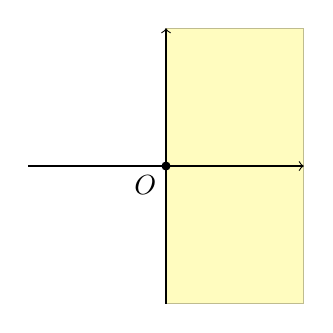
\begin{tikzpicture}
        %\draw[very thin,gray,step=0.5] (-1.75,-1.75) grid (1.75,1.75) ;
        \draw[fill=yellow,nearly transparent]
        (0,-1.75)--(0,1.75)--(1.75,1.75)--(1.75,-1.75)--cycle ;
        \draw[->] (-1.75,0) -- (1.75,0) ; % node[above]{$x$} ;
        \draw[->] (0,-1.75) -- (0,1.75) ; % node[right]{$y$} ;
        \draw[color=black,fill=black] (0,0) circle (0.05)
        node[below left] {$O$} ; 
      \end{tikzpicture}%
    }
    \only<3>{%
      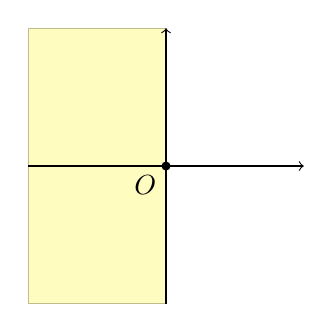
\begin{tikzpicture}
        %\draw[very thin,gray,step=0.5] (-1.75,-1.75) grid (1.75,1.75) ;
        \draw[fill=yellow,nearly transparent]
        (0,-1.75)--(0,1.75)--(-1.75,1.75)--(-1.75,-1.75)--cycle ;
        \draw[->] (-1.75,0) -- (1.75,0) ; % node[above]{$x$} ;
        \draw[->] (0,-1.75) -- (0,1.75) ; % node[right]{$y$} ;
        \draw[color=black,fill=black] (0,0) circle (0.05)
        node[below left] {$O$} ; 
      \end{tikzpicture}%
    }
    \only<4>{%
      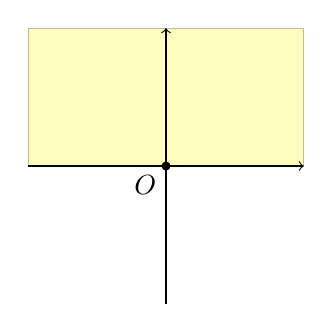
\begin{tikzpicture}
        %\draw[very thin,gray,step=0.5] (-1.75,-1.75) grid (1.75,1.75) ;
        \draw[fill=yellow,nearly transparent]
        (-1.75,0)--(1.75,0)--(1.75,1.75)--(-1.75,1.75)--cycle ;
        \draw[->] (-1.75,0) -- (1.75,0) ; % node[above]{$x$} ;
        \draw[->] (0,-1.75) -- (0,1.75) ; % node[right]{$y$} ;
        \draw[color=black,fill=black] (0,0) circle (0.05)
        node[below left] {$O$} ; 
      \end{tikzpicture}%
    }
    \only<5-6>{%
      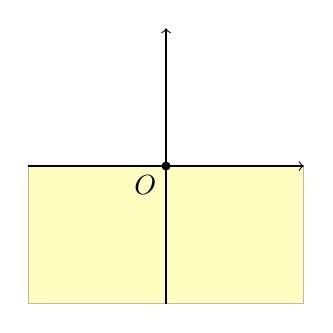
\begin{tikzpicture}
        %\draw[very thin,gray,step=0.5] (-1.75,-1.75) grid (1.75,1.75) ;
        \draw[fill=yellow,nearly transparent]
        (-1.75,0)--(1.75,0)--(1.75,-1.75)--(-1.75,-1.75)--cycle ;
        \draw[->] (-1.75,0) -- (1.75,0) ; % node[above]{$x$} ;
        \draw[->] (0,-1.75) -- (0,1.75) ; % node[right]{$y$} ;
        \draw[color=black,fill=black] (0,0) circle (0.05)
        node[below left] {$O$} ; 
      \end{tikzpicture}%
    }
    \only<7>{%
      \begin{tikzpicture}
        %\draw[very thin,gray,step=0.5] (-1.75,-1.75) grid (1.75,1.75) ;
        %\draw[fill=yellow,nearly transparent]
        %(0,0)--(0,1.75)--(1.75,1.75)--(1.75,0)--cycle ;
        \draw[->] (-1.75,0) -- (1.75,0) ; % node[above]{$x$} ;
        \draw[->] (0,-1.75) -- (0,1.75) ; % node[right]{$y$} ;
        \draw[color=black,fill=black] (0,0) circle (0.05)
        node[below left] {$O$} ; 
      \end{tikzpicture}%
    }
    \only<8>{%
      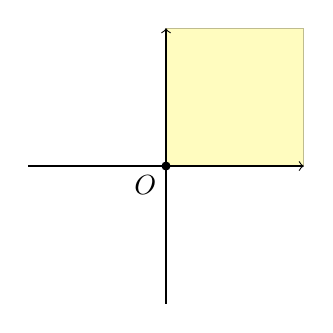
\begin{tikzpicture}
        %\draw[very thin,gray,step=0.5] (-1.75,-1.75) grid (1.75,1.75) ;
        \draw[fill=yellow,nearly transparent]
        (0,0)--(0,1.75)--(1.75,1.75)--(1.75,0)--cycle ;
        %\draw (-1.75/2,-1.75/2) node {$II$} ;
        \draw[->] (-1.75,0) -- (1.75,0) ; % node[above]{$x$} ;
        \draw[->] (0,-1.75) -- (0,1.75) ; % node[right]{$y$} ;
        \draw[color=black,fill=black] (0,0) circle (0.05)
        node[below left] {$O$} ; 
      \end{tikzpicture}%
    }
    \only<9>{%
      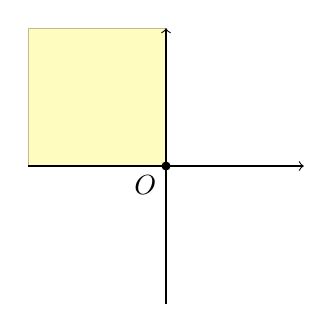
\begin{tikzpicture}
        %\draw[very thin,gray,step=0.5] (-1.75,-1.75) grid (1.75,1.75) ;
        \draw[fill=yellow,nearly transparent]
        (0,0)--(0,1.75)--(-1.75,1.75)--(-1.75,0)--cycle ;
        %\draw (-1.75/2,-1.75/2) node {$II$} ;
        \draw[->] (-1.75,0) -- (1.75,0) ; % node[above]{$x$} ;
        \draw[->] (0,-1.75) -- (0,1.75) ; % node[right]{$y$} ;
        \draw[color=black,fill=black] (0,0) circle (0.05)
        node[below left] {$O$} ; 
      \end{tikzpicture}%
    }
    \only<10>{%
      \begin{tikzpicture}
        %\draw[very thin,gray,step=0.5] (-1.75,-1.75) grid (1.75,1.75) ;
        \draw[fill=yellow,nearly transparent]
        (0,0)--(-1.75,0)--(-1.75,-1.75)--(-1.75,0)--cycle ;
        % EJD: grr (-0.825,-0.825) node {III} ;
        \draw[->] (-1.75,0) -- (1.75,0) ; % node[above]{$x$} ;
        \draw[->] (0,-1.75) -- (0,1.75) ; % node[right]{$y$} ;
        \draw[color=black,fill=black] (0,0) circle (0.05)
        node[below left] {$O$} ; 
      \end{tikzpicture}%
    }
    \only<11->{%
      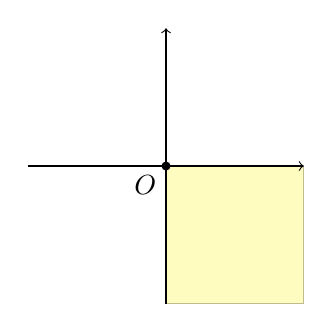
\begin{tikzpicture}
        %\draw[very thin,gray,step=0.5] (-1.75,-1.75) grid (1.75,1.75) ;
        \draw[fill=yellow,nearly transparent]
        (0,0)--(0,-1.75)--(1.75,-1.75)--(1.75,0)--cycle ;
        \draw[->] (-1.75,0) -- (1.75,0) ; % node[above]{$x$} ;
        \draw[->] (0,-1.75) -- (0,1.75) ; % node[right]{$y$} ;
        \draw[color=black,fill=black] (0,0) circle (0.05)
        node[below left] {$O$} ; 
      \end{tikzpicture}%
    }
  \end{columns}
\end{frame}

\begin{frame}
  \frametitle{Distance in the Cartesian Plane}
  \begin{columns}
    \column{0.65\textwidth}
    \begin{itemize}[<+->]
    \item<1-> Consider two points $P(x_1,y_1)$ and $Q(x_2,y_2)$ 
      in the Cartesian plane.
    \item<2-> We would like to find the distance between them.
    \item<3-> We add a ``construction point'' beside $P$ and below
      $Q$.
    \item<4-> We can easily find the distances from the $P$ to the
      construction point and from $Q$ to the construction point.
    \item<5-> We then use the Pythagorean Theorem to find the distance
      between $P$ and $Q$.
    \item<6-> The distance is $\sqrt{(x_2-x_1)^2+(y_2-y_1)^2}$
    \end{itemize}
    \column{0.35\textwidth}
    \only<1-2>{%
      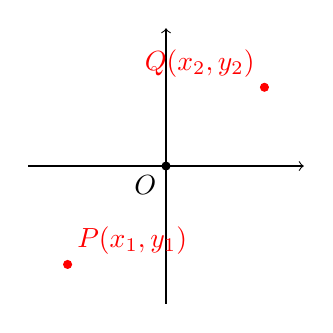
\begin{tikzpicture}
        %\draw[very thin,gray,step=0.5] (-1.75,-1.75) grid (1.75,1.75) ;
        \draw[->] (-1.75,0) -- (1.75,0) ; % node[above]{$x$} ;
        \draw[->] (0,-1.75) -- (0,1.75) ; % node[right]{$y$} ;
        \draw[color=black,fill=black] (0,0) circle (0.05)
        node[below left] {$O$} ; 
        \draw[color=red,fill=red] (-1.25,-1.25) circle (0.05)
        node[above right] {$P(x_1,y_1)$} ;
        \draw[color=red,fill=red] (1.25,1.00) circle (0.05) node[above left] {$Q(x_2,y_2)$} ;
      \end{tikzpicture}%
    }
    \only<3>{%
       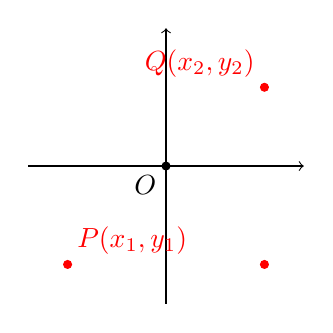
\begin{tikzpicture}
    %%     %\draw[very thin,gray,step=0.5] (-1.75,-1.75) grid (1.75,1.75) ;
         \draw[->] (-1.75,0) -- (1.75,0) ; % node[above]{$x$} ;
         \draw[->] (0,-1.75) -- (0,1.75) ; % node[right]{$y$} ;
         \draw[color=black,fill=black] (0,0) circle (0.05)
         node[below left] {$O$} ; 
         \draw[color=red,fill=red] (-1.25,-1.25) circle (0.05)
         node[above right] {$P(x_1,y_1)$} ;
         \draw[color=red,fill=red] (1.25,1.00) circle (0.05) node[above left] {$Q(x_2,y_2)$} ;
         \draw[color=red,fill=red] (1.25,-1.25) circle (0.05) ;
       \end{tikzpicture}%
    }
    \only<4>{%
       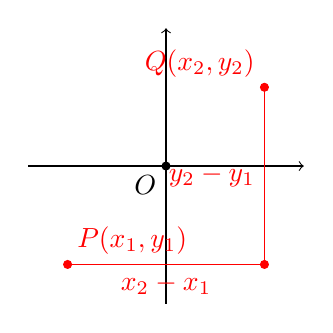
\begin{tikzpicture}
    %%     %\draw[very thin,gray,step=0.5] (-1.75,-1.75) grid (1.75,1.75) ;
         \draw[->] (-1.75,0) -- (1.75,0) ; % node[above]{$x$} ;
         \draw[->] (0,-1.75) -- (0,1.75) ; % node[right]{$y$} ;
         \draw[color=black,fill=black] (0,0) circle (0.05)
         node[below left] {$O$} ; 
         \draw[color=red,fill=red] (-1.25,-1.25) circle (0.05) node[above right] {$P(x_1,y_1)$} ;
         \draw[color=red,fill=red] (1.25,1.00) circle (0.05) node[above left] {$Q(x_2,y_2)$} ;
         \draw[color=red,fill=red] (1.25,-1.25) circle (0.05) ;
         \draw[color=red] (-1.25,-1.25)--(1.25,-1.25) node[midway,below] {$x_2-x_1$} ;
         \draw[color=red] (1.25,1.00)--(1.25,-1.25) node[midway,left] {$y_2-y_1$} ;
       \end{tikzpicture}%
    }
    \only<5->{%
       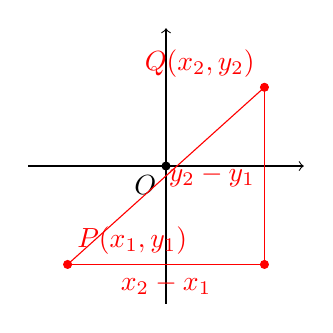
\begin{tikzpicture}
    %%     %\draw[very thin,gray,step=0.5] (-1.75,-1.75) grid (1.75,1.75) ;
         \draw[->] (-1.75,0) -- (1.75,0) ; % node[above]{$x$} ;
         \draw[->] (0,-1.75) -- (0,1.75) ; % node[right]{$y$} ;
         \draw[color=black,fill=black] (0,0) circle (0.05)
         node[below left] {$O$} ; 
         \draw[color=red,fill=red] (-1.25,-1.25) circle (0.05) node[above right] {$P(x_1,y_1)$} ;
         \draw[color=red,fill=red] (1.25,1.00) circle (0.05) node[above left] {$Q(x_2,y_2)$} ;
         \draw[color=red,fill=red] (1.25,-1.25) circle (0.05) ;
         \draw[color=red] (-1.25,-1.25)--(1.25,-1.25) node[midway,below] {$x_2-x_1$} ;
         \draw[color=red] (1.25,1.00)--(1.25,-1.25) node[midway,left] {$y_2-y_1$} ;
         \draw[color=red] (-1.25,-1.25)--(1.25,1.00) ;
       \end{tikzpicture}%
    }
  \end{columns}
\end{frame}


\subsection{Lines}

% EJD: graph of the meaning of the slopes?
% EJD: slope as rise/run?
\begin{frame}
  \frametitle{The Slope of a Line}
  \begin{columns}
    \column{0.65\textwidth}
    \begin{itemize}[<+->]
    \item Take any line on the plane.
    \item Pick two points on the line, $P(x_1,y_1)$ and $Q(x_2,y_2)$.
    \item As before, we find the construction point $R(x_2,y_1)$.
    \item Find the distance from $P$ to $R$, namely $x_2-x_1$
      and from $Q$ to $R$, namely $y_2-y_1$
    \item This time, we calculate their ratio:
      $\ds m = \frac{y_2-y_1}{x_2-x_1}$
    \item By similar triangles, that quantity depends only on the
      line.
    \item We call $m$ the \textit{slope} of the line.
    \end{itemize}
    \column{0.35\textwidth}
    \only<1>{
      \begin{tikzpicture}
         %\draw[very thin,gray,step=0.5] (-1.75,-1.75) grid (1.75,1.75) ;
         \draw[->] (-1.75,0) -- (1.75,0) ; % node[above]{$x$} ;
         \draw[->] (0,-1.75) -- (0,1.75) ; % node[right]{$y$} ;
         \draw[color=black,fill=black] (0,0) circle (0.05)
         node[below left] {$O$} ; 
         %\draw[color=red,fill=red] (-1.25,-1.25) circle (0.05) node[above right] {$P(x_1,y_1)$} ;
         %\draw[color=red,fill=red] (1.25,1.00) circle (0.05) node[above left] {$Q(x_2,y_2)$} ;
         %\draw[color=red,fill=red] (1.25,-1.25) circle (0.05) ;
         %\draw[color=red] (-1.25,-1.25)--(1.25,-1.25) node[midway,below] {$x_2-x_1$} ;
         %\draw[color=red] (1.25,1.00)--(1.25,-1.25) node[midway,left] {$y_2-y_1$} ;
         \draw[color=red] (-1.25,-1.25)--(1.25,1.00) ;
       \end{tikzpicture}%
    }
    \only<2>{
      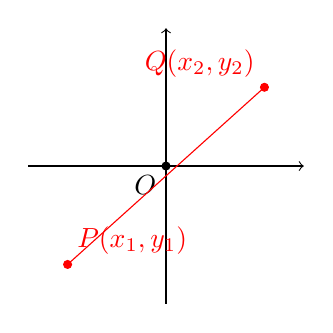
\begin{tikzpicture}
         %\draw[very thin,gray,step=0.5] (-1.75,-1.75) grid (1.75,1.75) ;
         \draw[->] (-1.75,0) -- (1.75,0) ; % node[above]{$x$} ;
         \draw[->] (0,-1.75) -- (0,1.75) ; % node[right]{$y$} ;
         \draw[color=black,fill=black] (0,0) circle (0.05)
         node[below left] {$O$} ; 
         \draw[color=red,fill=red] (-1.25,-1.25) circle (0.05) node[above right] {$P(x_1,y_1)$} ;
         \draw[color=red,fill=red] (1.25,1.00) circle (0.05) node[above left] {$Q(x_2,y_2)$} ;
         %\draw[color=red,fill=red] (1.25,-1.25) circle (0.05) ;
         %\draw[color=red] (-1.25,-1.25)--(1.25,-1.25) node[midway,below] {$x_2-x_1$} ;
         %\draw[color=red] (1.25,1.00)--(1.25,-1.25) node[midway,left] {$y_2-y_1$} ;
         \draw[color=red] (-1.25,-1.25)--(1.25,1.00) ;
       \end{tikzpicture}%
    }
    \only<3>{
      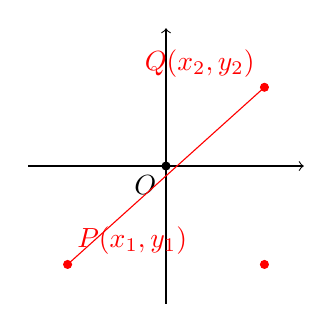
\begin{tikzpicture}
         %\draw[very thin,gray,step=0.5] (-1.75,-1.75) grid (1.75,1.75) ;
         \draw[->] (-1.75,0) -- (1.75,0) ; % node[above]{$x$} ;
         \draw[->] (0,-1.75) -- (0,1.75) ; % node[right]{$y$} ;
         \draw[color=black,fill=black] (0,0) circle (0.05)
         node[below left] {$O$} ; 
         \draw[color=red,fill=red] (-1.25,-1.25) circle (0.05) node[above right] {$P(x_1,y_1)$} ;
         \draw[color=red,fill=red] (1.25,1.00) circle (0.05) node[above left] {$Q(x_2,y_2)$} ;
         \draw[color=red,fill=red] (1.25,-1.25) circle (0.05) ;
         %\draw[color=red] (-1.25,-1.25)--(1.25,-1.25) node[midway,below] {$x_2-x_1$} ;
         %\draw[color=red] (1.25,1.00)--(1.25,-1.25) node[midway,left] {$y_2-y_1$} ;
         \draw[color=red] (-1.25,-1.25)--(1.25,1.00) ;
       \end{tikzpicture}%
    }
    \only<4>{
      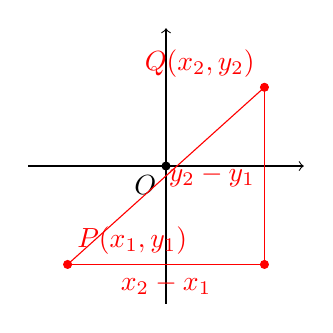
\begin{tikzpicture}
         %\draw[very thin,gray,step=0.5] (-1.75,-1.75) grid (1.75,1.75) ;
         \draw[->] (-1.75,0) -- (1.75,0) ; % node[above]{$x$} ;
         \draw[->] (0,-1.75) -- (0,1.75) ; % node[right]{$y$} ;
         \draw[color=black,fill=black] (0,0) circle (0.05)
         node[below left] {$O$} ; 
         \draw[color=red,fill=red] (-1.25,-1.25) circle (0.05) node[above right] {$P(x_1,y_1)$} ;
         \draw[color=red,fill=red] (1.25,1.00) circle (0.05) node[above left] {$Q(x_2,y_2)$} ;
         \draw[color=red,fill=red] (1.25,-1.25) circle (0.05) ;
         \draw[color=red] (-1.25,-1.25)--(1.25,-1.25) node[midway,below] {$x_2-x_1$} ;
         \draw[color=red] (1.25,1.00)--(1.25,-1.25) node[midway,left] {$y_2-y_1$} ;
         \draw[color=red] (-1.25,-1.25)--(1.25,1.00) ;
       \end{tikzpicture}%
    }
    \only<5->{
      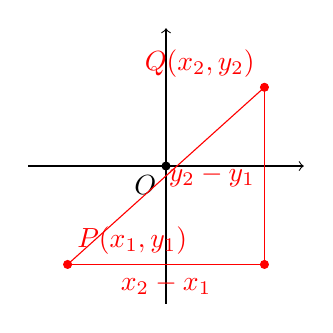
\begin{tikzpicture}
         %\draw[very thin,gray,step=0.5] (-1.75,-1.75) grid (1.75,1.75) ;
         \draw[->] (-1.75,0) -- (1.75,0) ; % node[above]{$x$} ;
         \draw[->] (0,-1.75) -- (0,1.75) ; % node[right]{$y$} ;
         \draw[color=black,fill=black] (0,0) circle (0.05)
         node[below left] {$O$} ; 
         \draw[color=red,fill=red] (-1.25,-1.25) circle (0.05) node[above right] {$P(x_1,y_1)$} ;
         \draw[color=red,fill=red] (1.25,1.00) circle (0.05) node[above left] {$Q(x_2,y_2)$} ;
         \draw[color=red,fill=red] (1.25,-1.25) circle (0.05) ;
         \draw[color=red] (-1.25,-1.25)--(1.25,-1.25) node[midway,below] {$x_2-x_1$} ;
         \draw[color=red] (1.25,1.00)--(1.25,-1.25) node[midway,left] {$y_2-y_1$} ;
         \draw[color=red] (-1.25,-1.25)--(1.25,1.00) ;
       \end{tikzpicture}%
    }
  \end{columns}
  % EJD: tidy up those diagrams ... use variables for P and Q
  % and stop it from jiggling!!
\end{frame}

% EJD: diagrams?
\begin{frame}
  \frametitle{Point-Slope Equation of a Line}
  \begin{columns}
    \column{0.65\textwidth}
    \begin{itemize}[<+->]
    \item Given a point $P$ and a point $Q$ on a line, we can figure
      out its slope $m$.
    \item On the other hand, given a point $P$ and the slope $m$, can
      we figure out \textit{all} the points $Q(x,y)$ that lie on the line?
    \item Yes, we just solve:
      \begin{equation*}
        m = \frac{y-y_1}{x-x_1} \implies y-y_1 = m(x-x_1)
      \end{equation*}
    \item That is the \textit{point-slope} form of the equation of a line.
    \end{itemize}
    \column{0.35\textwidth}
  \end{columns}
\end{frame}

% EJD: diagrms?
\begin{frame}
  \frametitle{Slope-Intercept Equation of a Line}
  \begin{columns}
    \column{0.65\textwidth}
    \begin{itemize}[<+->]
    \item A special case of the point-slope form of the equation of a
      line occurs when $P$ is a point on the $y$-axis.
    \item Such a point $P$ is called the \textit{$y$-intercept} of the
      line.
    \item In that case, $P(x_1,y_1)$ has the form $P(0,b)$.
    \item The equation of the line becomes
      \begin{equation*}
        y-b = m(x-0) \implies y=mx+b
      \end{equation*}
    \item We call that the \textit{slope-intercept} form of the
      equation of a line.
    \end{itemize}
    \column{0.35\textwidth}
  \end{columns}
\end{frame}

\begin{frame}
  \frametitle{Horizontal and Vertical Lines}
  \begin{columns}
    \column{0.65\textwidth}
    \begin{itemize}[<+->]
    \item The previous discussion holds for horizontal lines.
    \item In the case of a horizontal line, the slope is $m=0$.
    \item So the equation of a horizontal line is $y-y_1=0$
      (point-slope form) or $y=b$ (slope-intercept form).
    \item On the other hand, the slope of a vertical line is undefined
      (division by $0$).
    \item However, by analogy with the previous case, we can write an
      equation for a vertical line: $x=a$
    \end{itemize}
    \column{0.35\textwidth}
    \only<1-3>{ % horizontal line
      \begin{tikzpicture}
         %\draw[very thin,gray,step=0.5] (-1.75,-1.75) grid (1.75,1.75) ;
         \draw[->] (-1.75,0) -- (1.75,0) ; % node[above]{$x$} ;
         \draw[->] (0,-1.75) -- (0,1.75) ; % node[right]{$y$} ;
         \draw[color=black,fill=black] (0,0) circle (0.05)
         node[below left] {$O$} ; 
         \draw[red] (-1.75,0.75)--(1.75,0.75);
      \end{tikzpicture}
    }
    \only<4-5>{ % vertical line
      \begin{tikzpicture}
         %\draw[very thin,gray,step=0.5] (-1.75,-1.75) grid (1.75,1.75) ;
         \draw[->] (-1.75,0) -- (1.75,0) ; % node[above]{$x$} ;
         \draw[->] (0,-1.75) -- (0,1.75) ; % node[right]{$y$} ;
         \draw[color=black,fill=black] (0,0) circle (0.05)
         node[below left] {$O$} ; 
         \draw[red] (0.75,-1.75)--(0.75,1.75);
      \end{tikzpicture}
    }
  \end{columns}
\end{frame}

% EJD: diagrams?
\begin{frame}
  \frametitle{The General Equation of a Line}
  %\begin{columns}
    %\column{0.65\textwidth}
    \begin{itemize}[<+->]
    \item Sometimes we want an equation for a line that works for all
      lines, even vertical.
    \item The \textit{general equation of a line} $Ax+By+C=0$ works.
    \item We must have $A\ne 0$ or $B\ne 0$.  What happens if both $A=B=0$?
    \item Given point-slope form we can solve for general form:
      \begin{equation*}
        y-y_1 = m(x-x_1) \implies -mx + 1y + (mx_1-y_1) = 0
      \end{equation*}
    \item Given general form, with $B\ne 0$, we can solve for
      slope-intercept form:
      \begin{equation*}
        % EJD: highlight m and b
        Ax + By + C=0 \implies y = -\frac{A}{B} x - \frac{C}{B}
      \end{equation*}
    \item Given general form, with $B=0$, we can solve for
      vertical form:
      \begin{equation*}
        Ax + 0y + C = 0 \implies x = -\frac{C}{A}
      \end{equation*}
    \end{itemize}
    %\column{0.35\textwidth}
  %\end{columns}
\end{frame}

% EJD: diagrams
% EJD: highlight numbers that go into forming points
\begin{frame}
  \frametitle{Graphing Lines}
  \begin{columns}
    \column{0.65\textwidth}
    \begin{itemize}[<+->]
    \item To graph a line, 1) solve for $y$ then 2)
      substitute two different numbers for $x$ to get two points on
      the line.
    \item For example, consider $3x-2y=2$
    \item We solve for $y$: $y=(3/2)x-1$
    \item Choosing $x=0$ we get $y=(1/2)(0) - 1 = -1$ so
      $(0,-1)$ is a point on the line.
    \item Choosing $x=1$ we get $y=(3/2)(1) - 1 = 1/2$ so $(1,1/2)$ is
      a point on the line.
    \item Graph those points then draw a line through them.
    \end{itemize}
    \column{0.35\textwidth}
    \only<1-3>{ %
      \begin{tikzpicture}
         %\draw[very thin,gray,step=0.5] (-1.75,-1.75) grid (1.75,1.75) ;
         \draw[->] (-1.75,0) -- (1.75,0) ; % node[above]{$x$} ;
         \draw[->] (0,-1.75) -- (0,1.75) ; % node[right]{$y$} ;
         \draw[color=black,fill=black] (0,0) circle (0.05)
         node[below left] {$O$} ; 
      \end{tikzpicture}
    }
    \only<4>{ %
      \begin{tikzpicture}
         %\draw[very thin,gray,step=0.5] (-1.75,-1.75) grid (1.75,1.75) ;
         \draw[->] (-1.75,0) -- (1.75,0) ; % node[above]{$x$} ;
         \draw[->] (0,-1.75) -- (0,1.75) ; % node[right]{$y$} ;
         \draw[color=black,fill=black] (0,0) circle (0.05)
         node[below left] {$O$} ; 
         \draw[fill=red] (0,-1) circle (0.05);
      \end{tikzpicture}
    }
    \only<5>{ %
      \begin{tikzpicture}
         %\draw[very thin,gray,step=0.5] (-1.75,-1.75) grid (1.75,1.75) ;
         \draw[->] (-1.75,0) -- (1.75,0) ; % node[above]{$x$} ;
         \draw[->] (0,-1.75) -- (0,1.75) ; % node[right]{$y$} ;
         \draw[color=black,fill=black] (0,0) circle (0.05)
         node[below left] {$O$} ; 
         \draw[fill=red] (0,-1) circle (0.05);
         \draw[fill=red] (1,0.5) circle (0.05);
      \end{tikzpicture}
    }
    \only<6>{ %
      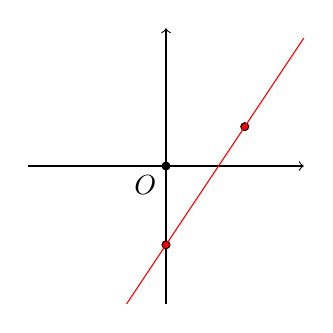
\begin{tikzpicture}
         %\draw[very thin,gray,step=0.5] (-1.75,-1.75) grid (1.75,1.75) ;
         \draw[->] (-1.75,0) -- (1.75,0) ; % node[above]{$x$} ;
         \draw[->] (0,-1.75) -- (0,1.75) ; % node[right]{$y$} ;
         \draw[color=black,fill=black] (0,0) circle (0.05)
         node[below left] {$O$} ; 
         \draw[fill=red] (0,-1) circle (0.05);
         \draw[fill=red] (1,1/2) circle (0.05);
         \draw[color=red] (-0.5,-1.75)--(1.75,1.625);
      \end{tikzpicture}
    }
  \end{columns}
\end{frame}

% EJD: two examples, one with $\ge$ and one with $>$
\begin{frame}
  \frametitle{Graphing Linear Inequalities}
  \begin{columns}
    \column{0.65\textwidth}
    \begin{itemize}[<+->]
    \item We follow a similar pattern to graph a linear inequality.
    \item Consider $3x-2y>2$
    \item Solve for $y$: $y<(3/2)x-1$
    \item Note the change in direction of the inequality!
    \item The $<$ means the line itself is not included in the graph,
      so we draw a dashed line.
    \item The $<$ also means we take all points below the line.
    \end{itemize}
    \column{0.35\textwidth}
    \only<1-4>{ %
      \begin{tikzpicture}
         %\draw[very thin,gray,step=0.5] (-1.75,-1.75) grid (1.75,1.75) ;
         \draw[->] (-1.75,0) -- (1.75,0) ; % node[above]{$x$} ;
         \draw[->] (0,-1.75) -- (0,1.75) ; % node[right]{$y$} ;
         \draw[color=black,fill=black] (0,0) circle (0.05)
         node[below left] {$O$} ; 
         %\draw[fill=red] (0,-1) circle (0.05);
         %\draw[fill=red] (1,1/2) circle (0.05);
         %\draw[color=red] (-0.5,-1.75)--(1.75,1.625);
      \end{tikzpicture}
    }
    \only<5>{ %
      \begin{tikzpicture}
         %\draw[very thin,gray,step=0.5] (-1.75,-1.75) grid (1.75,1.75) ;
         \draw[->] (-1.75,0) -- (1.75,0) ; % node[above]{$x$} ;
         \draw[->] (0,-1.75) -- (0,1.75) ; % node[right]{$y$} ;
         \draw[color=black,fill=black] (0,0) circle (0.05)
         node[below left] {$O$} ; 
         %\draw[fill=red] (0,-1) circle (0.05);
         %\draw[fill=red] (1,1/2) circle (0.05);
         \draw[color=red,dashed] (-0.5,-1.75)--(1.75,1.625);
      \end{tikzpicture}
    }
    \only<6>{ %
      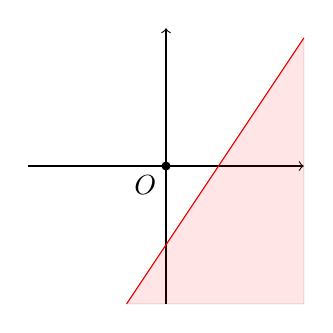
\begin{tikzpicture}
         %\draw[very thin,gray,step=0.5] (-1.75,-1.75) grid (1.75,1.75) ;
         \draw[->] (-1.75,0) -- (1.75,0) ; % node[above]{$x$} ;
         \draw[->] (0,-1.75) -- (0,1.75) ; % node[right]{$y$} ;
         \draw[color=black,fill=black] (0,0) circle (0.05)
         node[below left] {$O$} ; 
         %\draw[fill=red] (0,-1) circle (0.05);
         %\draw[fill=red] (1,1/2) circle (0.05);
         \draw[color=red] (-0.5,-1.75)--(1.75,1.625);
         \draw[fill=red,very nearly transparent] (-0.5,-1.75) -- (1.75,-1.75) %
         -- (1.75,1.625) -- cycle;
      \end{tikzpicture}
    }
  \end{columns}
\end{frame}


\subsection{Relationships Between Lines}

% EJD: diagrams
\begin{frame}
  \frametitle{Parallel and Perpendicular Lines}
  \begin{columns}
    \column{0.65\textwidth}
    \begin{itemize}[<+->]
    \item Sometimes we need to deal with two lines
      \begin{equation*}
        \mbox{$y = m_1 x + b_1$ \quad and \quad $y = m_2 x + b_2$}
      \end{equation*}
    \item We would like to detect relationships between them.
    \item They are parallel iff slopes are the same:
      \begin{equation*}
        \mbox{parallel} \Leftrightarrow m_1=m_2
      \end{equation*}
    \item They are perpendicular iff slopes are negative reciprocal:
      \begin{equation*}
        \mbox{perpendicular} \Leftrightarrow m_1 = -1/m_2
      \end{equation*}
    \end{itemize}
    \column{0.35\textwidth}
    \only<3>{ %
      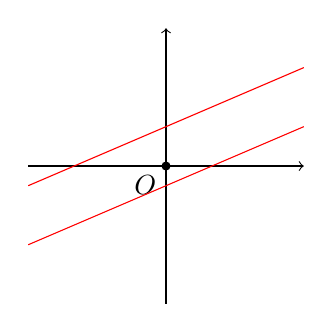
\begin{tikzpicture}
         %\draw[very thin,gray,step=0.5] (-1.75,-1.75) grid (1.75,1.75) ;
         \draw[->] (-1.75,0) -- (1.75,0) ; % node[above]{$x$} ;
         \draw[->] (0,-1.75) -- (0,1.75) ; % node[right]{$y$} ;
         \draw[color=black,fill=black] (0,0) circle (0.05)
         node[below left] {$O$} ; 
         \draw[color=red] (-1.75,-1.00)--(1.75,0.5);
         \draw[color=red] (-1.75,-0.25)--(1.75,1.25);
      \end{tikzpicture}
    }
    \only<4>{ %
      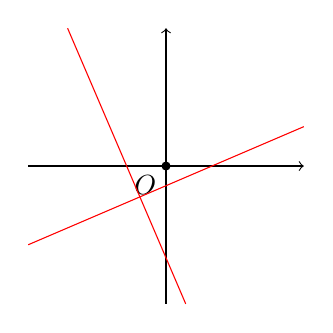
\begin{tikzpicture}
         %\draw[very thin,gray,step=0.5] (-1.75,-1.75) grid (1.75,1.75) ;
         \draw[->] (-1.75,0) -- (1.75,0) ; % node[above]{$x$} ;
         \draw[->] (0,-1.75) -- (0,1.75) ; % node[right]{$y$} ;
         \draw[color=black,fill=black] (0,0) circle (0.05)
         node[below left] {$O$} ; 
         \draw[color=red] (-1.75,-1)--(1.75,0.5);
         \draw[color=red] (0.25,-1.75)--(-1.25,1.75);
      \end{tikzpicture}
    }
  \end{columns}
\end{frame}

% EJD: diagrams
\begin{frame}
  \frametitle{Parallel Lines}
  \begin{columns}
    \column{0.65\textwidth}
    \begin{itemize}[<+->]
    \item Suppose I want to find a line through $(5,3)$
      that is parallel to $x-2y=2$
    \item The given line in slope-intercept form is $y=(1/2)x-1$
      so its slope is $1/2$
    \item The unknown line is parallel to the given line, so the slope
      of the unknown line is also $1/2$
      % EJD: emphasize *also*
    \item By point-slope form the equation of the unknown line is
      $y-3=(1/2)(x-5)$
      % EJD: show again where 3, 5, and 1/2 came from
    \end{itemize}
    \column{0.35\textwidth}
  \end{columns}
\end{frame}

% EJD: diagrams
\begin{frame}
  \frametitle{Perpendicular Lines}
  \begin{columns}
    \column{0.65\textwidth}
    \begin{itemize}[<+->]
    \item On the other hand suppose I want to find a line through $(5,3)$
      that is perpendicular to $x-2y=2$
    \item The given line in slope-intercept form is $y=(1/2)x-1$
      so its slope is $1/2$
    \item The unknown line is \textit{perpendicular} to the given
      line, so the slope of the unknown line is $-1/(1/2)=-2$.
      % EJD: emphasize *also*
    \item By point-slope form an equation of the unknown line is
      $y-3=-2(x-5)$
      % EJD: show again where 3, 5, and -2 came from
    \end{itemize}
    \column{0.35\textwidth}
  \end{columns}
\end{frame}


\end{document}

